\chapter{Local Dependencies}
\label{cha:SL}

\begin{itemize}
    \item closure under complementation
    \item think of grammars as constraints/dependencies; can we combine dependencies? yes, closure under intersection
    \item characterization in terms of substring substitution closure
    \item generalization to n-grams; many follow-up exercises
    \item cognitive and learnability implications for local dependencies
\end{itemize}

\section{Phonological Processes as Lists}
Let's return to the specific phenomenon of final devoicing for a moment.
This process can be captured by straying not too far from our idea of phonology as a list, but without running into the issues the latter faces.
In order to verify that a word satisfies word-final devoicing, it suffices to look at the very last allophone;
the word is phonologycally well-formed only if the last sound is not voiced.
Since every language has only a finite number of allophones, we can write a list of allophones that may occur in word-final position, and those that may not.
%
\begin{center}
    \begin{tabular}{r@{\hskip 2em}ccccc}
        \textbf{word-final}     & p & t & k & s & \ldots\\
        \textbf{not word-final} & b & d & g & z & \ldots
    \end{tabular}
\end{center}
%
This list will vary between languages, but it fully characterizes which sounds may occur at the end of a word.

But final devoicing is only one of myriads of local processes in phonology, so unless the idea above can easily be generalized to other local processes it is of very little practical use.
Remember, treating phonology as a list of word pronunciations may not be elegant or enlightening, but at least it is guaranteed to always yield correct output forms.

Consider a simple process like nasal assimilation in English, where a nasal consonant (\textipa{m}, \textipa{n}, \textipa{\ng}) that is followed by a plosive (\textipa{p}, \textipa{b}, \textipa{t}, \textipa{d}, \textipa{k}, \textipa{g}) changes into the nasal whose place of articulation is closest to that of the plosive.
For instance, \textipa{/b\ae nk/} is pronounced \textipa{b\ae\ng k} --- the alveolar \textipa{n} turns into velar \textipa{\ng} by virtue of \textipa{k} being velar.
In this case we can also write a list, but we need more than two categories.
%
\begin{center}
    \begin{tabular}{r@{\hskip 2em}c}
        \textbf{before \textipa{p} or \textipa{b}} & \textipa{m}\\
        \textbf{before \textipa{t} or \textipa{d}} & \textipa{n}\\
        \textbf{before \textipa{k} or \textipa{g}} & \textipa{\ng}\\
    \end{tabular}
\end{center}
%
This list is not quite correct however, because plosives can be preceded by sounds besides nasals.
So a more accurate listing would also need to contain vowels and other consonants.
%
\begin{center}
    \begin{tabular}{r@{\hskip 2em}cccc}
        \textbf{before \textipa{p} or \textipa{b}} & \textipa{m}   & \textipa{a} & \textipa{s} & \ldots\\
        \textbf{before \textipa{t} or \textipa{d}} & \textipa{n}   & \textipa{a} & \textipa{s} & \ldots\\
        \textbf{before \textipa{k} or \textipa{g}} & \textipa{\ng} & \textipa{a} & \textipa{s} & \ldots\\
    \end{tabular}
\end{center}

It looks like we now have list-based accounts for two distinct processes, but how can we be sure that the two are actually similar accounts?
For instance, the following list should strike you as a lot stranger than the previous two.
%
\begin{center}
    \begin{tabular}{r@{\hskip 2em}ccccc}
        \textbf{after a perfect number of sounds}     & \textipa{p} & \textipa{t} & \textipa{k} & \textipa{z} & \ldots\\
        \textbf{after an imperfect number of sounds} & \textipa{b} & \textipa{d} & \textipa{g} & \textipa{s} & \ldots\\
    \end{tabular}
\end{center}
%
A \emph{perfect number} is a number that is identical to the sum of its remainder-free divisors, e.g.\ $6 = 1 + 2 + 3$ or $28 = 1 + 2 + 4 + 7 + 14$.
The list above, then, tells us that certain consonants may be voiced iff their position in the word is a perfect number.
Of course no natural language behaves like that.
Consequently we need an explanation as to why the first two kinds of lists are phonologically natural, whereas the third one is not.

The most obvious answer is that there is a difference in how these lists pick out positions.
The first two regulate the shape of a sound depending on what it is followed by.
The nasalization process can easily be compiled out into a list of well-formed sequences of two sounds: \textipa{mp}, \textipa{mb}, \textipa{nt}, \textipa{nd}, \textipa{\ng k}, \textipa{\ng g}, \textipa{ap}, \textipa{ab}, and so on.
We call such sequences of two sounds \emph{bigrams}.
Crucially the list does not contain bigrams like \textipa{nk}, so a word where \textipa{n} is followed by \textipa{k} is not phonologically well-formed.
The same compiling-out procedure can be used for word-final devoicing if we use the special symbol $\RightEdgeSymbol$ to mark the end of the word.
The list contains the bigrams \textipa{p\RightEdge}, \textipa{t\RightEdge}, \textipa{k\RightEdge}, \textipa{s\RightEdge}, but not \textipa{b\RightEdge}, \textipa{d\RightEdge}, \textipa{g\RightEdge}, or \textipa{z\RightEdge}.
Thus the first two processes share the property that they can be described via a finite list of bigrams.

The hypothetical perfect-number phenomenon, on the other hand, cannot be described in terms of bigrams.
A sequence like \textipa{ap} is licit in the string XXX, but illicit in \textipa{tRap}. %fixme: example string
The way sounds are regulated no longer depends on adjacency to a specific sound but rather a highly abstract counting mechanism.
So one idea we may explore for now is that all phonological processes can be captured via finite lists of bigrams.
In other words, phonology is a bigram grammar.

\section{Bigram Grammars and Recognizers}

\subsection{The Intuition Behind Bigram Grammars}
A \emph{bigram grammar} is a just finite set of bigrams.
Each bigram encodes a licit sequence of two sounds.
So a bigram grammar $G$ considers a string $w$ well-formed iff every sequence of two adjacent symbols in $w$ is a bigram of $G$.
We refer to these sequences as bigrams, too.
In other words, a string is well-formed iff it consists only of bigrams that are licensed by the grammar.
We also say that the bigram grammar \emph{generates} this string.

\begin{examplebox}[Strings licensed by a small bigram grammar]
    \label{ex:SL_BigramGrammar}%
    Suppose grammar $G$ contains the bigrams $\LeftEdge a$, $\mathit{ab}$, $b \RightEdge$, where $\LeftEdgeSymbol$ and $\RightEdgeSymbol$ mark the left and right edge of the string, respectively.
    Now consider the string $\mathit{ab}$, which we may also write $\LeftEdge \mathit{ab} \RightEdge$ for the sake of explicitness.
    This string consists of the bigrams $\LeftEdge a$, $\mathit{ab}$, and $b \RightEdge$.
    Since all of those bigrams are part of $G$, the string is well-formed. 

    The minimally different $\mathit{ba}$, on the other hand, is built from the bigrams $\LeftEdge b$, $\mathit{ba}$, and $\mathit{a \RightEdge}$.
    Not a single one of those bigrams is contained in $G$, and consequently $G$ does not generate this string.

    The string $\mathit{abb}$ is not generated by $G$ either.
    Even though three of its bigrams are part of $G$ --- namely $\LeftEdge a$, $\mathit{ab}$, and $b \RightEdge$ --- its fourth bigram $\mathit{bb}$ is not among $G$'s bigrams.
    So even though 75\% of this string's bigrams are well-formed, it is still not generated by the grammar.
    A single mistake is enough to render it illicit.

    Notice that $G$ only generates the finite language $\setof{\mathit{ab}}$.
    Suppose that we extend $G$ so that it also generates $\mathit{abab}$.
    This requires adding the bigram $\mathit{ba}$ to $G$.
    But this allows $G$ not only to generate the string $\mathit{abab}$, but also $\mathit{ababab}$, $\mathit{abababab}$, and so on.
    The addition of a single bigram pushed the language generated by $G$ from a finite one to an infinite one.
    We also see that not all finite languages can be generated by bigram languages.
    Any attempt to do so yields an infinite superset of the finite language.
\end{examplebox}

\subsection{Recognition via a Bigram Scanner}
A subtle point that is easy to lose sight of is that the grammar is just a specification of which strings are well-formed, it does not include a procedure for verifying whether a given string is actually well-formed.
That is easy to see if we think about how we would implement a bigram grammar in Python.
Given the definition above, a bigram grammar is simply a set of bigrams.
This is straight-forwardly translated into Python.
%
\pythonfile[firstline=4,lastline=4]{./code/bigram_scanner/bigram_scanner_set_unsafe.py}
%
Clearly the definition of a variable is not enough to produce a useful program.
What we need is a mechanism that takes the grammar as a parameter and then determines if a given string is generated by the grammar.
Such a mechanism is called a \emph{recognizer} as it recognizes whether a string is well-formed.

There's many different ways one may construct a recognizer, but for a bigram grammar the simplest model is that of a \emph{scanner}.
The scanner has a window that is exactly two symbols wide.
It moves this window through the string from left to right, and at each step it checks whether the sequence of symbols it sees in its window is part of the bigram grammar (see Fig.~\ref{fig:SL_Scanner} for an illustration).
If the answer is no, it rejects the string.
Otherwise it moves the window one symbol further to the right.
If the window cannot be moved further to the right, the scanner accepts the string as well-formed.
%
\begin{figure}[tbph]
\centering
\begin{tikzpicture}
    \begin{scope}[spy using outlines={rectangle, size = 5em}]
        % input string    
        \foreach \Name/\Symbol in { 0/$\LeftEdgeSymbol$,
                                    1/$a$,
                                    2/$b$,
                                    3/$a$,
                                    4/$b$,
                                    5/$a$,
                                    6/$b$,
                                    7/$a$,
                                    8/$b$,
                                    9/$b$,
                                    10/$\RightEdgeSymbol$
                                  }
            \node[text height=.75em] (\Name) at ($(\Name*1.5em,0)$) {\Symbol};

        % arrow for scanner direction
        \draw[blue,->] (2.north) to (7.north);

        % list of bigrams
        \node (bigrams) at (5.south)
            [
            yshift=-12em,
            minimum width=7em,
            minimum height=7.5em,
            fill=red!5,
            draw=red,
            thick,
            rounded corners
            ]
            {%
                \begin{tabular}{l}
                    \\[-.5em]
                    $\LeftEdge a$\\
                    $\mathit{ab}$\\
                    $\mathit{ba}$\\
                    $b \RightEdge$
                \end{tabular}%
            };

        % name of list of bigrams
        \node (G) at (bigrams.north)
            [
            minimum width=7em,
            fill=red,
            draw=red,
            thick,
            rounded corners
            ]
            {\color{white}\textbf{Grammar}};

        % frame for looking up first scanned bigram 
        \draw[thick,gray,fill=gray!50,opacity=.3] ($(bigrams.west)+(1em,2em)$) rectangle ($(bigrams.east)+(-1em,1em)$);

        % frame for failed looked up of second scanned bigram
        \node[xshift=3em,yshift=-2em, thick,draw=gray,fill=gray!50,opacity=.3,align=center] (failed) at (bigrams.east) {\phantom{error}};
        \node at (failed) {error};

        % first scanner window
        %---------------------
        % create center coordinate for zoom target
        \coordinate (zoomcenter-good) at ($(0.east) !.5! (1.west)$);

        % spy on zoom target, create node (zoom) below
        \spy[magnification=2,
             blue,
             spy connection path={
                \draw[dashed] (tikzspyonnode.north west) -- (tikzspyinnode.north west);
                \draw[dashed] (tikzspyonnode.north east) -- (tikzspyinnode.north east);
                \draw[dashed] (tikzspyonnode.south west) -- (tikzspyinnode.south west);
                \draw[dashed] (tikzspyonnode.south east) -- (tikzspyinnode.south east);
                \draw[dashed,gray] (tikzspyinnode.south) ..
                                            controls +(245:8em) and +(170:3em) ..
                                                ($(bigrams.west)+(1em,1.5em)$);
            }]
            on (zoomcenter-good) in node [fill=blue!5] (zoom-good) at ($(zoomcenter-good) - (0,5em)$);


        % second scanner window
        %----------------------
        % create center coordinate for zoom target
        \coordinate (zoomcenter-bad) at ($(8.east) !.5! (9.west)$);

        % spy on zoom target, create node (zoom) below
        \spy[magnification=2,
             blue,
             spy connection path={
                \draw[dashed] (tikzspyonnode.north west) -- (tikzspyinnode.north west);
                \draw[dashed] (tikzspyonnode.north east) -- (tikzspyinnode.north east);
                \draw[dashed] (tikzspyonnode.south west) -- (tikzspyinnode.south west);
                \draw[dashed] (tikzspyonnode.south east) -- (tikzspyinnode.south east);
                \draw[dashed,gray] (tikzspyinnode.south) ..
                                            controls +(300:6em) and +(30:6em) ..
                                                (failed.east);
            }]
            on (zoomcenter-bad) in node [fill=blue!5] (zoom-bad) at ($(zoomcenter-bad) - (0,5em)$);

    \end{scope}
\end{tikzpicture}

\caption{Scanner for a bigram grammar}
\label{fig:SL_Scanner}
\end{figure}

Notice that the scanner as described above queries the grammar during every step it takes through the string.
This is somewhat wasteful --- after all, if we've already verified once that $\mathit{ab}$ is a licit bigram, why should we have to do so again at a later point.
An alternative is to first move the scan window through the entire string while keeping track of the bigrams one encounters.
That way one obtains the set of all bigrams in the string (note that no bigram occurs more than once in this set).
Once the scanning steps have concluded, we simply check whether the set of bigrams is a subset of the grammar.
If that is not the case, then the string contains some bigram that is not part of the grammar, so we are dealing with an ill-formed string. 
Otherwise the string is well-formed.
A Python implementation of this approach is given in~\ref{code:SL_SetScanner}.

\begin{listing}[tbph]
\pythonfile[firstline=7]{./code/bigram_scanner/bigram_scanner_set_unsafe.py}
\caption{Python implementation of a set-based scanner}
\label{code:SL_SetScanner}
\end{listing}


\subsection{Positive and Negative Bigram Grammars}

Contemporary phonology does not think of phenomena like final devoicing as a process but rather as a constraint: certain sounds are banned from occurring word-finally.
This can be represented as below using an Optimality Theory (OT) tableau.
%
\begin{center}
    \begin{tabular}{r|c}
        \textipa{/rad/} & $^*$[+voice]$\RightEdge$\\
        \hline
        \textipa{[rad]} & !* \\
        \textipa{[rat]} &
    \end{tabular}
\end{center}
%
Similarly, assimilation is nowadays analyzed as the result of a ban against certain sound sequences.

This constraint-based perspective can be accommodated in a very natural way in the bigram framework.
Right now, we interpret the bigrams of a grammar as licit sequences, that is, a string is well-formed iff all its bigrams are licensed by the grammar. 
But we could also view things the other way round such that the grammar's bigrams list illicit sequences.
Each bigram then encodes a specific constraint of the grammar, and consequently a string is well-formed iff none of its bigrams are listed by the grammar.
We call these two types of bigram grammars \emph{positive} and \emph{negative}, respectively.
%
\begin{examplebox}[A negative bigram grammar]
    Consider once more the bigram grammar $G$ from the beginning of example~\ref{ex:SL_BigramGrammar}, which consisted of the bigrams $\LeftEdge a$, $\mathit{ab}$, and $b \RightEdge$.
    As a positive bigram grammar, $G$ generates only the string $\mathit{ab}$.
    As a negative bigram grammar, it generates all strings that
    %
    \begin{itemize*}
        \item do not start with an $a$, and
        \item do not end in a $b$, and
        \item do not contain an $a$ followed by $b$.
    \end{itemize*}
    %
    Notice that this set is infinite, as it contains the strings $\mathit{ba}$, $\mathit{bba}$, $\mathit{bbba}$, and so on.
\end{examplebox}

Now that we have two different ways of interpreting bigram grammars, the obvious question is whether the two differ in any respect.
In particular, is one more powerful than the other?
This is a challenging question, after all there are infinitely many grammars of each type, so we can't just compare them one by one.
What we need is a way to talk about these two infinite classes of grammars in a precise and rigorous manner.
We need math.


\section{Mathematics of Bigram Grammars}

\subsection{Equivalence of Positive and Negative Bigram Grammars}

Mathematics and its tools require a certain amount of precision and explicitness, with respect to concepts as well as notation.
This is not too different from programming, where you have to use the correct syntax, define your variables and functions, and so on.
In many respects math is actually less verbose and pedantic because it allows us to abstract away from details that aren't relevant for our purposes (for instance what kind of data structure to use for sets).
While we have been fairly explicit about bigram grammars, it is nonetheless prudent to make all our terms fully explicit before moving on.

\begin{definition}[Strings]
    A \emph{string alphabet} is a finite, non-empty set of symbols.
    We usually drop the ``string'' part and simply speak of alphabets.
    A \emph{string} over alphabet $\Sigma$ is a finite sequence of symbols drawn from $\Sigma$.
    Given two strings $u$ and $v$, we denote by $u \stringcat v$ the \emph{concantenation} of the two, which is the string $uv$.
    The \emph{empty string} $\emptystring$ is the unique string that contains no symbols.
\end{definition}
%
Some scholars would consider this definition of string still too sloppy since we did not specify what we mean by a sequence of symbols.
For our purposes the definition is good enough, but if you're curious here's a more technical one: a string over $\Sigma$ is an initial subset of the natural numbers with a labeling function $\LabelFunc$ from $\NatNum$ to $\Sigma$.
This definition exploits the fact that the natural numbers are string-like (1 before 2, 2 before 3, 3 before 4) and then simply a symbol from $\Sigma$ to the first $n$ natural numbers as their label.

Quite generally, mathematical objects can be defined in many different ways.
This is not a pointless exercise, very often a good definition is the most important step towards discovering new facts about an object.
In fact, if you can think of only one way to define an object, that is a clear-cut sign that you do not understand the object very well.
\citet[10]{KeenanMoss12} express this succinctly yet with the appropriate force:
%
\begin{center}
    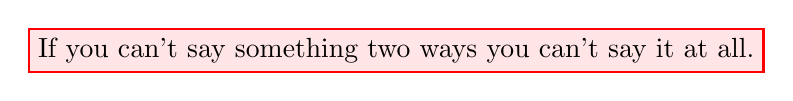
\begin{tikzpicture}
        \node[draw=red, fill=red!10, thick]
            {If you can't say something two ways you can't say it at all.};
    \end{tikzpicture}
\end{center}

This credo may seem odd to linguists, who usually take a strongly realist stance according to which the grammar formalism fully specifies the grammar, even down to notation.
For example, SPE and OT are regarded as vastly different theories that describe diametrically opposed conceptions of phonology.
Yet we will see at a later point that they are but two definitions of the same computational object.
That does not rule out that one of the two is a more useful way of thinking about phonology, but that is a matter of epistemology rather than ontology.

\begin{definition}[Bigrams]
    Given a string $w$ over alphabet $\Sigma$, its \emph{augmented} counterpart $\augmented{w} \is \LeftEdge \stringcat w \stringcat \RightEdge$ is obtained by adding the left and right edge markers $\LeftEdge$ and $\RightEdge$ to $w$, where $\LeftEdge$ and $\RightEdge$ are distinguished symbols not contained in $\Sigma$.
    Furthermore, 
    \(
    \Bigrams(w) \is
        \setof{
            ab \mid \exists u,v  \text{ s.t.\ } u \stringcat ab \stringcat v = \augmented{w}
        }
    \)
    denotes the set of \emph{bigrams} over $\augmented{w}$, i.e.\ the smallest set that contains all substrings of $\augmented{w}$ that consist of exactly $2$ symbols.
\end{definition}

\begin{definition}[Bigram Grammar]
    A \emph{bigram grammar} $G$ over alphabet $\Sigma$ is a finite set of bigrams over $\Sigma \cup \setof{\LeftEdge, \RightEdge}$.
    If $G$ is a \emph{positive bigram grammar} (denoted $\posG{G}$), then it generates the language
    \(
        L(G) \is \setof{
            w \mid \Bigrams(w) \subseteq G
        }
    \).
    If $G$ is a \emph{negative bigram grammar} (denoted $\negG{G}$), then it generates the language
    \(
        L(G) \is \setof{
            w \mid \Bigrams(w) \cap G = \emptyset
        }
    \).
\end{definition}

With all these definitions under our belt, we can finally move on to producing a new insight: positive and negative bigram grammars are equally powerful.
That is to say, if some language is generated by a positive bigram grammar, then it can also be generated by some negative bigram grammar, and the other way round.

\begin{theorem}
    The class of languages that are generated by positive bigram grammars is exactly the class of languages that are generated by negative bigram grammars.
    \label{thm:SL_PosNegEquivalence}
\end{theorem}
%
In order to show that this theorem is indeed correct, we establish two simpler propositions --- called lemmata --- which jointly imply the theorem.

\begin{lemma}
    For every positive bigram grammar there is a negative bigram grammar that generates the same language.
    \label{lem:SL_Pos2Neg}
\end{lemma}
%
\begin{proof}
    Let $\posG{G}$ be a positive bigram grammar. 
    We show that $\negG{\complementof{G}}$ defines the same language as $\posG{G}$, where $\complementof{G}$ consists of all bigrams over $\Sigma \cup \setof{\LeftEdge, \RightEdge}$ that are not contained by $G$.

    Pick some arbitrary string $w \in L(\posG{G})$. 
    By definition, every bigram of $w$ is a member of $G$, which immediately implies that no element of $\Bigrams(w)$ is contained in $\complementof{G}$.
    But if none of the bigrams of $w$ belong to $\complementof{G}$, then $\Bigrams(w) \cap \complementof{G} = \emptyset$, wherefore $w \in L(\negG{\complementof{G}})$.
    Since $w$ was arbitrary, this result holds for every string generated by $\posG{G}$, establishing $L(\posG{G}) \subseteq L(\negG{\complementof{G}})$.

    The same argument can be applied in the other direction to show $L(\posG{G}) \supseteq L(\negG{\complementof{G}})$, wherefore $L(\posG{G}) = L(\negG{\complementof{G}})$.
\end{proof}
%
This is a so-called \emph{constructive} proof: we do not just show that an equivalent negative bigram grammar exists, we also explain how this grammar can be constructed from the positive bigram grammar.
Constructive proofs are the most useful kind of proof because they provide procedures and strategies that can be implemented and run automatically.

In the case at hand, all we have to do in order to construct an equivalent negative bigram grammar is to take the set-theoretic complement of the positive bigram grammar.
After all, the set of all bigrams over $\Sigma$ is given by $\Sigma \times \Sigma$, and the positive bigram grammar $\posG(G)$ is some subset thereof (\emph{modulo} edge markers, which are treated as part of $\Sigma$ here to avoid notational clutter).
Bigrams that belong to $G$ may occur in a string, bigrams that do not must not.
So the bigrams not belonging to $G$ are the illicit bigrams, which means those are exactly the bigrams the equivalent negative bigram grammar must contain.
In one sentence: taking the complement of $G$ is like taking its negation, and the switch from a positive grammar to a negative one undoes this negation.

So now we know that the negative bigram grammars are at least as powerful as the positive bigram grammars since the latter can be translated into the former.
It only remains for us to show that the same holds in the other direction.

\begin{lemma}
    For every negative bigram grammar there is a positive bigram grammar that generates the same language.
\end{lemma}
%
\begin{proof}
    Left as an exercise to the reader.
\end{proof}

\subsection{The How and Why of Proofs}

Proofs are a difficult art at every level of expertise.
For the beginner, the biggest challenge is often to sort out their train of thought and present it in a clear manner: where do I start, and how do I proceed from there step by step to reach the conclusion?

There are no clear-cut rules here, but it is often helpful to break up the problem into smaller ones, as we did with Thm.~\ref{thm:SL_PosNegEquivalence}.
If two sets $A$ and $B$ need to be shown to be equivalent, one can first prove $A \subseteq B$ and then $B \subseteq A$.
And a statement of the form ``$\phi$ iff $\psi$'' can be broken up into ``$\phi$ entails $\psi$'' and ``$\psi$ entails $\phi$''.
We will encounter several basic proof techniques throughout the course (proof by induction, indirect proofs), but don't worry too much about specific techniques for now.
Instead, make sure to work through the proofs we discuss multiple times until you understand how they work.
Always try to answer the following questions for yourself:

\begin{itemize}
    \item Why is the initial assumption valid?
    \item How does each conclusion follow from the previous one?
    \item Why does the final conclusion show that the theorem\slash lemma is correct?
\end{itemize}

You may wonder why we need proofs in the first place.
Linguists don't work with proofs yet they have discovered a lot of interesting things about language.
Programmers don't have much use for proofs either.
There's several answers, the simplest one being that some questions can only be addressed conclusively via proofs.
Consider the following alternative to the proof of Lem.~\ref{lem:SL_Pos2Neg}: we could have implemented the translation procedure from positive to negative grammars and then tested it on a large sample of positive bigram grammars (at least several thousand).
Eventually the program would have told us that the negative grammars generate the same string languages as their positive counterparts.
So if the conversion works correctly on every single one of thousands of positive bigram grammars, isn't that enough to posit that positive and negative bigram grammars are interchangeable?

The answer is No.
First of all, checking that two grammars generate the same language is hardly trivial if both languages are infinite (we can't just compare all their respective members).
More importantly, though, the thousands of test grammars may accidentally share a special property that is essential for the correctness of the conversion.
This is a real risk if all those test grammars were automatically generated by a script because true randomness is very hard to achieve with computers, if not impossible.
While experiments and simulations have their place --- they are a valid last resort where proofs are hard to come by --- a proof is always the preferred solution where possible.

Proofs are preferred not only because they are safe from the pitfalls of simulations, but also because they provide genuine insight.
In fact, proofs are often more important and enlightening than the theorems they establish.
Testing the correctness of the bigram conversion via automated experiments could at best show us whether the procedure is correct (if there's only finitely many cases to test), but it does not tell us \textbf{why}.
A proof is an explicit record of how certain properties entail others.
In the case at hand, it is the close connection between set-theoretic complementation and the switch from positive to negative grammars that does all the work.
Notice all the properties of bigram grammars that the proof does not depend on: that bigrams are strings, that bigrams consist of exactly two symbols, and that bigram grammars are finite. 
Yet these properties necessarily hold during any test procedure, so we would not be able to tell which one of them is a prerequisite for the correctness of the conversion.
Thanks to the proof, we know which properties matter, which in turn might come in handy in the study of other formalisms.

In a few lines, a proof can establish unassailable truths, show us why they hold, but also save us hours of work compared to running simulations.
So even though you may initially find them hard and time consuming, proofs are actually the tool of choice for the lazy scientist.


\subsection{Basic Closure Properties}

\begin{lemma}
    The class of bigram languages is closed under intersection.
\end{lemma}
%
\begin{proof}
    We prove that for any two bigram languages generated by (positive) bigram grammars $G_1$ and $G_2$, $L(G_1) \cap L(G_2) = L(G_1 \cap G_2)$.
    We first show $L(G_1) \cap L(G_2) \subseteq L(G_1 \cap G_2)$.
    Let $w$ be an arbitrary string belonging to both $L(G_1)$ and $L(G_2)$, i.e.\ $w \in L(G_1) \cap L(G_2)$.
    Then every bigram of $w$ is contained in both $G_1$ and $G_2$, so $w \in L(G_1 \cap G_2)$.
    Since $w$ is arbitrary, we have $L(G_1) \cap L(G_2) \subseteq L(G_1 \cap G_2)$.
    The same reasoning can be applied in the other direction, yielding $L(G_1 \cap G_2) \subseteq L(G_1) \cap L(G_2)$.
    These two facts jointly imply $L(G_1) \cap L(G_2) = L(G_1 \cap G_2)$.
\end{proof}
%
% hw: spell out the second subset relation

\begin{lemma}
    The class of bigram languages is not closed under union. 
\end{lemma}
%
\begin{proof}
    We give an example of two bigram languages whose union is not a bigram language.
    Let $L_1 \is \setof{\mathit{ab}}$ and $L_2 \is \setof{\mathit{b}, \mathit{bb}, \mathit{bbb}, \ldots}$.
    Assume without loss of generality (w.l.o.g.) that all bigram grammars are positive.
    Then any bigram grammar that generates $L_1$ must contain the bigrams $\LeftEdge a$, $\mathit{ab}$, and $b \RightEdge$.
    Similarly, a bigram grammar generating $L_2$ must contain the bigrams $\LeftEdge b$, $\mathit{bb}$, and $b \RightEdge$.
    Therefore a bigram grammar that generates all strings in $L_1 \cup L_2$ must contain at least these bigrams.
    But such a grammar also generates the string $\mathit{abb}$, which is not part of $L_1 \cup L_2$.
    Hence there is no bigram grammar that generates all the strings in $L_1 \cup L_2$ and nothing else, so $L_1 \cup L_2$ is not a bigram language.
\end{proof}
%
%hw: extend proof to case where both languages are infinite

\begin{lemma}
    The class of bigram languages is not closed under (relative) complement.
\end{lemma}
%
\begin{proof}
    This is an immediate consequence of the previous lemmata and what is called De Morgan's law: $L_1 \cup L_2 = \complementof{\complementof{L_1} \cap \complementof{L_2}}$.
    If the class of bigram languages were closed under both complement and intersection, it would be closed under union, too.
    Since closure under union does not hold, closure under intersection or complement must fail.
    We have already seen that closure under intersection holds, so closure under complement cannot hold, too.
\end{proof}
%
%hw: give a proof by example
Slightly surprising because we have the option to take complements of grammars, but that's not string language complements.

\begin{lemma}
    The class of bigram languages is not closed under relabelings.
\end{lemma}
%
\begin{proof}
    Consider the language $L \is \setof{\mathit{ab}, \mathit{abab}, \mathit{ababab}, \ldots}$ and the relabeling $r$ that replaces all $b$s by $a$s.
    The image of $L$ under $r$ consists of all strings that contain a (positive) even number of $a$s and nothing else: $\mathit{aa}$, $\mathit{aaaa}$, $\mathit{aaaaaa}$, and so on.
    Every such string contains the bigrams $\LeftEdge a$, $\mathit{aa}$, and $a \RightEdge$.
    But a grammar with these bigrams also generates the strings $a$, $\mathit{aaa}$, $\mathit{aaaaa}$, and so on, which shows that the image of $L$ under $r$ cannot be generated by a bigram grammar.
    Consequently, closure under relabelings does not hold for the class of bigram languages.
\end{proof}
%
ties into abstractness debate (e.g. if we have hidden C-V layer, language is definable).

\subsection{Substring Substitution Closure}

\subsection{\texorpdfstring{Generalization to $n$-Gram Grammars}{Generalization to n-Gram Grammars}}

\section{Implications for Phonology}

%hw: implement a negative bigram grammar
%hw: implement translation from positive into negative bigram grammar

local substring substitution

%hw: what happens if we run our scanner with grammar for {LR} and string LLLRRR; is this accepted? why? how to fix the issue?
%hw: scanner is not psycholinguistically plausible (incrementality)
%hw: is memory usage a good argument for online scanner?
